\documentclass[a4paper]{report}

\usepackage[T1]{fontenc}
\usepackage[utf8]{inputenc}
\usepackage[english]{babel}

\usepackage{color,soul}
\usepackage{longtable}
\usepackage{amsmath}
\usepackage{booktabs}
\usepackage{rotating}

\renewcommand{\arraystretch}{1.2}

\usepackage{hyperref}

% Display code - main interest is it can import external files
\usepackage{listings}
\usepackage[usenames]{xcolor}

\usepackage{svg}

% Custom style for the code
\lstset{
	commentstyle=\color{gray},
	tabsize=4,
	basicstyle={\small\ttfamily}
}

% TiKZ for the drawings
\usepackage{tikz}
\usetikzlibrary{shapes}

\setlength{\textwidth}{16cm} \setlength{\textheight}{23cm}
\setlength{\oddsidemargin}{0cm} % +0.5 si {\textwidth}{15cm} ; -0,5 si {\textwidth}{15cm}
\setlength{\headheight}{0cm} \setlength{\topmargin}{0.3cm}
\setlength{\headsep}{0cm}

% Deletes the chapters and uses roman numbers for the sections
\usepackage{chngcntr}
\counterwithout{section}{section}
\renewcommand{\thesection}{\Roman{section}}
\renewcommand{\thesubsection}{\thesection.\arabic{subsection}}
\renewcommand{\thesubsubsection}{\thesection.\arabic{subsection}.\alph{subsubsection}}

\author{Clément Decoodt, Alexis Bauvin, Alexandre Janniaux}
\title{PR1 SE201: execution platforms}

\begin{document}

\maketitle

The aim of this project was to implemet a simple ALU and engineer a simple
\emph{friendly} processor with its instrution set and pipeline.

ALU is programmed in C and would simulate the behavior of a real ALU by
operating directly on the bits. The objective was to properly do all operations
without using C operators.

The instruction set is very limited but sufficient to do basic programs (and
surely more advanced). It mimics the MIPS instruction set, and being very
limited, it probably is a RISC processor.

\section{Two's complement arithmetic}

\subsection{Unsigned addition}

	In this part, we implemented an unsigned adder using full adders made of half adders. Each adder was made entirely by logical operators in the file available in \href{https://github.com/friendshipismagic/friendly-computing-machine/blob/master/proj1/src/addition.c}{addition.c source file}. \\
	
	Chosen endianness is little endian to get a more natural operator reading and parsing (left to right). \\
	
	Useful inputs are available in the \href{https://github.com/friendshipismagic/friendly-computing-machine/blob/master/proj1/src/tests.c}{tests file}. The Unit test framework tests for the following events in the unsigned adder :

\begin{center}
	\begin{tabular}{|l|l|l|}
		\hline
		Test & Expected result & Tested event \\
		\hline \hline
		10000 + 10000 & 01000 & Carry check \\
		00010 + 00001 & 00011 & Basic test \\
		11110 + 11110 & 01111 & Yet another basic test \\
		00001 + 00010 & 00011 & Basic commutativity check \\
		00110 + 00010 & 00101 & Commutativity check with carry \\
		00010 + 00110 & 00101 & Same as above \\
		10101 + 11100 & 00111 & Random test (Just in case)\\
		11111 + 10000 & 00000 & Overflow test \\
		\hline
	\end{tabular}
\end{center}

	For both the full and half adder, every input is tested as these are 1 bit only. \\

\subsection{Signed addition}

	In this part, we implemented a signed adder using two's complement method: inputs are first 1-complemented, them both are summed as unsigned, and finally the result is 1-complemented. An event is raised in case of overflow. To check for overflow we just needed to see if adding two same-signed numbers result in opposed-signed number. The tests are also available in tests file. They're mainly:

\begin{center}
	\begin{tabular}{|l|l|l|}
		\hline
		Test & Expected result & Tested event \\
		\hline \hline
		00000 + 00000 & 00000 & Complement basic error check \\
		11111 + 10000 & 00000 & Endianness check \\
		10000 + 10000 & 01000 & Tests for unsigned addition \\
		00000 + 11111 & 11111 & Zero test \\
		11111 + 11111 & 01111 & Negative test \\
		00001 + 00001 & 00000 & Overflow test \\
		\hline
	\end{tabular}
\end{center}

\subsection{Subtraction minus one}

	The subtraction minus one is just an addition with the second input one's complemented to get $-B-1$ instead of $B$. Same basic tests as for unsigned addition are done.

\subsection{Multiplication}

	The multiplier is made of an adder and a for loop. Zeroes and ones are immediatly treated to avoid entering in the loop. Tests are:

\begin{center}
	\begin{tabular}{|l|l|l|}
		\hline
		Test & Expected result & Tested event \\
		\hline \hline
		0x0 * 0x0 & 0x0 & Zero optimisation \\
		0x1 * 0x1 & 0x1 & One optimisation \\
		0x2 * 0x2 & 0x4 & Basic multiplication \\
		0x1337 * 0x2 & 0x1337<<1 & Another basic multiplication \\
		0xFFFFFFFF * 0xFFFFFFFF & overflow & Overflow test \\
		\hline
	\end{tabular}
\end{center}

\subsection{Multiplication and overflow}

\subsubsection{Multiplication}

Numbers are chosen randomly. $X=10100$ and $Y=11001$.

\begin{center}
	\begin{longtable}{|c|c|l|}
		\hline
		Iterator & Product register & Operations \\
		\hline \hline
		0        & 0             & Load Multiplicand and product register \\
		\hline \hline
		0        & 1010000000    & Add 1 to iterator, load $X$ in product register, load next multiplicand \\
		\hline
		         & ~~~1010000000 & Add-accumulate product register with $X$ as multiplicand is $1$ \\
		1        &  +~1010000000 & load new multiplicand, increase iterator \\
		         &  =~0101000000 & and branch if iterator equals $Y$ \\
		\hline                  
		         & ~~~0101000000 & Don't add to product register \\
		10       &  +~1010000000 & load new multiplicand, increase iterator \\
		         &  =~1111000000 & Do not branch (iterator not equal to $Y$) \\
		\hline                  
		         & ~~~1111000000 & Don't add to product register \\
		11       &  +~1010000000 & load new multiplicand, increase iterator \\
		         &  =~0010100000 & Do not branch (iterator not equal to $Y$) \\
		\hline                  
		         & ~~~0010100000 & Add-accumulate product register with $X$ as multiplicand is $1$ \\
		100      &  +~1010000000 & load new multiplicand, increase iterator \\
		         &  =~1001100000 & Do not branch (iterator not equal to $Y$) \\
		\hline \hline           
		         & ~~~1001100000 & Add-accumulate product register with $X$ as multiplicand is $1$ \\
		101      &  +~1010000000 & load new multiplicand, increase iterator \\
		         &  =~0111100000 & Do not branch (iterator not equal to $Y$) \\
		\hline                  
		         & ~~~0111100000 & Add-accumulate product register with $X$ as multiplicand is $1$ \\
		110      &  +~1010000000 & load new multiplicand, increase iterator \\
		         &  =~1100010000 & Do not branch (iterator not equal to $Y$) \\
		\hline                  
		         & ~~~1100010000 & Don't add to product register \\
		111      &  +~1010000000 & load new multiplicand, increase iterator \\
		         &  =~0001010000 & Do not branch (iterator not equal to $Y$) \\
		\hline                  
		         & ~~~0001010000 & Don't add to product register \\
		1000     &  +~1010000000 & load new multiplicand, increase iterator \\
		         &  =~1011010000 & Do not branch (iterator not equal to $Y$) \\
		\hline                  
		         & ~~~1011010000 & Add-accumulate product register with $X$ as multiplicand is $1$ \\
		1001     &  +~1010000000 & load new multiplicand, increase iterator \\
		         &  =~0100110000 & Do not branch (iterator not equal to $Y$) \\
		\hline \hline           
		         & ~~~0100110000 & Add-accumulate product register with $X$ as multiplicand is $1$ \\
		1010     &  +~1010000000 & load new multiplicand, increase iterator \\
		         &  =~1110110000 & Do not branch (iterator not equal to $Y$) \\
		\hline                  
		         & ~~~1110110000 & Add-accumulate product register with $X$ as multiplicand is $1$ \\
		1011     &  +~1010000000 & load new multiplicand, increase iterator \\
		         &  =~0011110000 & Do not branch (iterator not equal to $Y$) \\
		\hline                  
		         & ~~~0011110000 & Don't add to product register \\
		1100     &  +~1010000000 & load new multiplicand, increase iterator \\
		         &  =~1000001000 & Do not branch (iterator not equal to $Y$) \\
		\hline                  
		         & ~~~1000001000 & Don't add to product register \\
		1101     &  +~1010000000 & load new multiplicand, increase iterator \\
		         &  =~0110001000 & Do not branch (iterator not equal to $Y$) \\
		\hline                  
		         & ~~~0110001000 & Add-accumulate product register with $X$ as multiplicand is $1$ \\
		1110     &  +~1010000000 & load new multiplicand, increase iterator \\
		         &  =~1101001000 & Do not branch (iterator not equal to $Y$) \\
		\hline \hline           
		         & ~~~1101001000 & Add-accumulate product register with $X$ as multiplicand is $1$ \\
		1111     &  +~1010000000 & load new multiplicand, increase iterator \\
		         &  =~0000101000 & Do not branch (iterator not equal to $Y$) \\
		\hline                  
		         & ~~~0000101000 & Add-accumulate product register with $X$ as multiplicand is $1$ \\
		10000    &  +~1010000000 & load new multiplicand, increase iterator \\
		         &  =~1010101000 & Do not branch (iterator not equal to $Y$) \\
		\hline                  
		         & ~~~1010101000 & Don't add to product register \\
		10001    &  +~1010000000 & load new multiplicand, increase iterator \\
		         &  =~0101101000 & Do not branch (iterator not equal to $Y$) \\
		\hline                  
		         & ~~~0101101000 & Don't add to product register \\
		10010    &  +~1010000000 & load new multiplicand, increase iterator \\
		         &  =~1111101000 & Do not branch (iterator not equal to $Y$) \\
		\hline                  
		         & ~~~1111101000 & Add-accumulate product register with $X$ as multiplicand is $1$ \\
		10011    &  +~1010000000 & load new multiplicand, increase iterator \\
		         &  =~0010011000 & Do not branch (iterator not equal to $Y$) \\
		\hline \hline           
		         & ~~~0010011000 & Add-accumulate product register with $X$ as multiplicand is $1$ \\
		10100    &  +~1010000000 & load new multiplicand, increase iterator \\
		         &  =~1001011000 & Do not branch (iterator not equal to $Y$) \\
		\hline                  
		         & ~~~1001011000 & Add-accumulate product register with $X$ as multiplicand is $1$ \\
		10101    &  +~1010000000 & load new multiplicand, increase iterator \\
		         &  =~0111011000 & Do not branch (iterator not equal to $Y$) \\
		\hline                  
		         & ~~~0111011000 & Don't add to product register \\
		10110    &  +~1010000000 & load new multiplicand, increase iterator \\
		         &  =~1100111000 & Do not branch (iterator not equal to $Y$) \\
		\hline                  
		         & ~~~1100111000 & Don't add to product register \\
		10111    &  +~1010000000 & load new multiplicand, increase iterator \\
		         &  =~0001111000 & Do not branch (iterator not equal to $Y$) \\
		\hline                  
		         & ~~~0001111000 & Add-accumulate product register with $X$ as multiplicand is $1$ \\
		11000    &  +~1010000000 & load new multiplicand, increase iterator \\
		         &  =~1011111000 & Do not branch (iterator not equal to $Y$) \\
		\hline \hline           
		11001    & 0  1011111000 & Iterator equals $Y$, this is the end! \\
		\hline

	\end{longtable}
\end{center}

\subsubsection{Overflow determination}

Let's declare $v$ where
$$\left\lbrace
\begin{array}{lr}
	v(1>>n) = n+1 \\
	v(1>>n + 1>>m) = max(v(n),v(m)) + (n==m) \\
	\forall a,b \neq 0 : v(a*b) = v(a) + v(b)
\end{array}\right.
$$

So, overflow condition is $v(a*b) \leq N+1$, meaning $v(a)+v(b) \leq 6$

\subsubsection{Example}

Chosen $A=00001$ and $B=01000$ (little endian), we can check for overflow: $v(A*B)=v(A)+v(B)=5 + 2 \geq 6$ \\
We overflow here! In fact, the result is $A*B=000001$ which is not storable on a 5-bit number.

\section{Processor design}

\subsection{Instruction set architecture}

We defined our architecture set instruction as the following:

\subsubsection{R-type instructions}

Instruction structure :

\begin{center}
	\begin{tabular}{|l|l|l|l|}
		\hline
		opcode & output register & input register 1 & input register 2 \\
		\hline
		7 bits & 3 bits & 3 bits & 3 bits \\
		\hline
	\end{tabular}
\end{center}

Instruction list :

\begin{center}
	\begin{tabular}{|l|l|l|}
		\hline
		Opcode & Mnemonic & Description \\
		\hline \hline
		\texttt{0000000} & \texttt{NOP} &  Does nothing \\
		\texttt{0000011} & \texttt{ADD} &  Adds two signed numbers \\
		\texttt{0000111} & \texttt{ADDU} & Adds two unsigned numbers \\
		\texttt{0000010} & \texttt{SUB} &  Substracts two signed numbers \\
		\texttt{0000110} & \texttt{SUBU} & Substracts two unsigned numbers \\
		\texttt{0000100} & \texttt{MULU} & Multiplied two unsigned numbers \\
		\hline
	\end{tabular}
\end{center}

Example:

\texttt{sub \$r1 \$r2 \$r3} : computes \texttt{\$r2} $-$ \texttt{\$r3} and stores the
result in \texttt{\$r1}. \\
Encodes to ${
	\underbrace{\texttt{0000010}}_{opcode}
	\underbrace{\texttt{001}}_{out}
	\underbrace{\texttt{010}}_{in 1}
	\underbrace{\texttt{011}}_{in 2}\mbox{}_2 % The mbox serves to add another subscript
}$ = \texttt{0x0453}$_{16}$

\subsubsection{I-type instructions}

Instruction structure :

\begin{center}
	\begin{tabular}{|l|l|l|}
		\hline
		opcode & output register & immediate value \\
		\hline
		2 bits & 3 bits & 11 bits \\
		\hline
	\end{tabular}
\end{center}

Instruction list :

\begin{center}
	\begin{tabular}{|l|l|l|}
		\hline
		Opcode & Mnemonic & Description \\
		\hline \hline
		\texttt{10} & \texttt{ADDIU} & Adds-accumulate an unsigned immediate
		                               value to output register \\
		\texttt{11} & \texttt{LWI} &   Copies the immediate value to
		                               the register \\
		\hline
	\end{tabular}
\end{center}

Example:

\texttt{addiu \$r6 420h} : computes \texttt{\$r6} $+$ \texttt{0x420} and stores
the result in \texttt{\$r6}. \\
Encodes to ${
	\underbrace{\texttt{10}}_{opcode}
	\underbrace{\texttt{110}}_{out}
	\underbrace{\texttt{10000100000}}_{value}\mbox{}_2
}$ = \texttt{0xb420}$_{16}$

\subsubsection{J-type instructions}

Instruction structure :

\begin{center}
	\begin{tabular}{|l|l|l|l|}
		\hline
		opcode & register 1 & register 2 & immediate value \\
		\hline
		4 bits & 3 bits & 3 bits & 6 bits \\
		\hline
	\end{tabular}
\end{center}

Instruction list :

\begin{center}
	\begin{tabular}{|l|l|l|}
		\hline
		Opcode & Mnemonic & Description \\
		\hline \hline
		\texttt{0010} & \texttt{LW} & Loads word from memory at address
		                              \texttt{\$r2 + immediate} (offset) into \\
		              &             & first register \\
		\texttt{0011} & \texttt{SW} & Stores word in \texttt{\$r1} to memory at
		                           address \texttt{\$r2 + immediate} (offset) \\
		\hline
	\end{tabular}
\end{center}

Example: if \texttt{\$r2} contains \texttt{0x1337},

\texttt{lw \$r1 \$r2 0x2a} : reads the word at address \texttt{\$r2} +
\texttt{0x2a} (i.e. \texttt{0x1361}) and stores it in \texttt{\$r1} \\
Encodes to ${
	\underbrace{\texttt{0010}}_{opcode}
	\underbrace{\texttt{001}}_{out}
	\underbrace{\texttt{010}}_{adr}
	\underbrace{\texttt{101010}}_{offset}\mbox{}_2
}$ = \texttt{0x22aa}$_{16}$

\subsubsection{K-type instructions}

Instruction structure :

\begin{center}
	\begin{tabular}{|l|l|l|l|}
		\hline
		opcode & immediate value & register 1 & register 2 \\
		\hline
		2 bits & 8 bits & 3 bits & 3 bits \\
		\hline
	\end{tabular}
\end{center}

Instruction list :

\begin{center}
	\begin{tabular}{|l|l|l|}
		\hline
		Opcode & Mnemonic & Description \\
		\hline \hline
		\texttt{01} & \texttt{BNE} & Jumps to \texttt{pc + immediate} if
		                             \texttt{\$r1 $\neq$ \$r2} \\
		\hline
	\end{tabular}
\end{center}

Example:

\texttt{bne -3h \$r1 \$r5} : compares \texttt{\$r1} and \texttt{\$r5} and
jumps to \texttt{\$pc + immediate} if they are different \\
Encodes to ${
	\underbrace{\texttt{01}}_{opcode}
	\underbrace{\texttt{11111101}}_{offset}
	\underbrace{\texttt{001}}_{reg 1}
	\underbrace{\texttt{101}}_{reg 1}\mbox{}_2
}$ = \texttt{0x7f4d}$_{16}$

\subsubsection{Instruction tree}

We are using a binary tree to determine the actual instruction :

\begin{center}
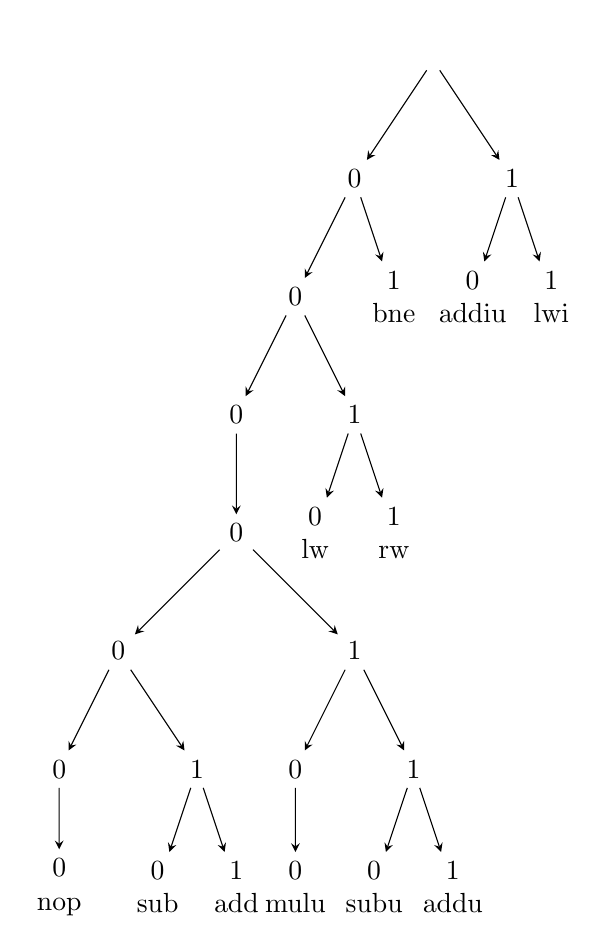
\begin{tikzpicture}[>=stealth]
	\tikzstyle{every node}=[align=center]
	\tikzstyle{level 1}=[sibling distance=20mm]
	\tikzstyle{level 2}=[sibling distance=10mm]
	\tikzstyle{level 4}=[sibling distance=10mm]
	\tikzstyle{level 5}=[sibling distance=30mm]
	\tikzstyle{level 6}=[sibling distance=20mm]
	\tikzstyle{level 7}=[sibling distance=10mm]
	\node {} [->]
		child {node {0}
			child[sibling distance=15mm] {node {0}
				child[sibling distance=15mm] {node {0}
					child {node {0}
						child {node {0}
							child[sibling distance=15mm] {node {0}
								child {node {0\\nop}}
							}
							child {node {1}
								child {node {0\\sub}}
								child {node {1\\add}}
							}
						}
						child {node {1}
							child[sibling distance=15mm] {node {0}
								child {node {0\\mulu}}
							}
							child[sibling distance=15mm] {node {1}
								child {node {0\\subu}}
								child {node {1\\addu}}
							}
						}
					}
				}
				child {node {1}
					child {node {0\\lw}}
					child {node {1\\rw}}
				}
			}
			child {node {1\\bne}}
		}
		child {node {1}
			child {node {0\\addiu}}
			child {node {1\\lwi}}
		}
	;
\end{tikzpicture}
\end{center}

\subsubsection{Assembly samples}

We will assume here that the assembler supports labels for the jumps -- which
the included Javascript one does.

\mbox{}\\
The following code will load the constant $2^{21}$ into the register
\texttt{\$r1} :
\lstinputlisting[language={[x86masm]Assembler}]{../src/two_pow_21.s}
To avoid the use of labels, it is equivalent to write \texttt{-2h} in
place of \texttt{loop} in the \texttt{bne} instruction.

\mbox{}\\
This is the correspondance between a bit of C code and its compiled
version :

% The tabular forces the codes to be on the same height
\noindent\begin{tabular}{cc}
	\begin{lstlisting}[language=C]
int *a = 0x200;
int s = 0;
for (int i = 0; i != 10; i++) {
	s = s + *a;
	a++;
}
\end{lstlisting}
	&
	\lstinputlisting[language={[x86masm]Assembler}]{../src/c_code.s}
\end{tabular}

\subsection{Pipelining}

\subsubsection{Pipelined processor}

Pipelined processor is drawn here. Actual hazards can be:

\begin{itemize}
	\item Data hazard, when a branch should be followed based on a register being calculated on the ALU \\
	\item Control hazard, when a branch is going to happen the two next operation can be forwarded and flushed (wrong branch prediction)
	\item If a lw and a sll happens on the same register, this register will be accessed at the same time
\end{itemize}

A basic solution is to stall. Forwarding cannot occur as we would need a 5-stage processor to enable forwarding (there is no MEM or WB stage here). Flushing can be used to help resolve control hazard.

\begin{sidewaysfigure}
	\centering
	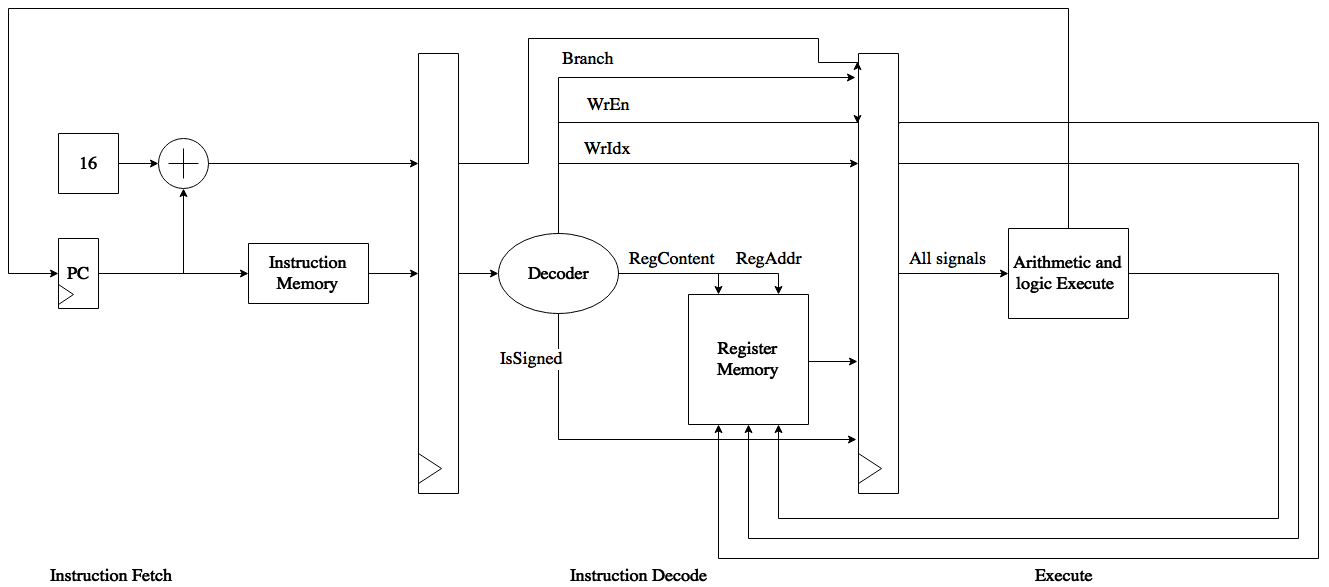
\includegraphics[width=25cm]{processor.png}
\end{sidewaysfigure}

\subsubsection{Pipelined diagram}

\begin{sidewaysfigure}
	\begin{longtable} {|l|c|c|c|c|c|c|c|c|c|c|c|c|c|c|c|c|c|c|c|}
		\hline
		LW          & IF & ID & EX &    &    &    &    &    &    &    &    &    &    &    &    &    &    &    &    \\ \hline
		\hl{ADD}    &    & IF & ID & ID & EX &    &    &    &    &    &    &    &    &    &    &    &    &    &    \\ \hline
		ADDIU       &    &    & IF & IF & ID & EX &    &    &    &    &    &    &    &    &    &    &    &    &    \\ \hline
		SUB         &    &    &    &    & IF & ID & EX &    &    &    &    &    &    &    &    &    &    &    &    \\ \hline
		\hl{BNE}    &    &    &    &    &    & IF & ID & ID & EX &    &    &    &    &    &    &    &    &    &    \\ \hline
		\hl{NOP}    &    &    &    &    &    &    & -- & -- & -- & -- &    &    &    &    &    &    &    &    &    \\ \hline
		\hl{NOP}    &    &    &    &    &    &    &    &    & -- & -- & -- &    &    &    &    &    &    &    &    \\ \hline
		LW          &    &    &    &    &    &    &    &    &    & IF & ID & EX &    &    &    &    &    &    &    \\ \hline
		\hl{ADD}    &    &    &    &    &    &    &    &    &    &    & IF & ID & ID & EX &    &    &    &    &    \\ \hline
		ADDIU       &    &    &    &    &    &    &    &    &    &    &    & IF & IF & ID & EX &    &    &    &    \\ \hline
		SUB         &    &    &    &    &    &    &    &    &    &    &    &    &    & IF & ID & EX &    &    &    \\ \hline
		\hl{BNE}    &    &    &    &    &    &    &    &    &    &    &    &    &    &    & IF & ID & ID & EX &    \\ \hline
		\hl{NOP}    &    &    &    &    &    &    &    &    &    &    &    &    &    &    &    & -- & -- & -- & -- \\ \hline
		\hl{NOP}    &    &    &    &    &    &    &    &    &    &    &    &    &    &    &    &    &    & -- & -- \\ \hline
	\end{longtable}
\end{sidewaysfigure}

\begin{itemize}
	\item \textit{ADD} and \textit{BNE} are data hazards, as they're waiting for previous instruction to write the right value to the register file. \\
	\item \textit{NOP} instructions are here because of the control hazard generated by the \textit{BNE} instructions (there is no branch prediction so branches are not taken by default)

\end{itemize}

\end{document}


